%%%%%%%%%%%%%%%%%%%%%%%%%%%%%%%%%%%%%%%%%
% Beamer Presentation
% Standard LaTeX Template used for creating presentation of Firebird-V Robot and other tutorials. 
% Author: (e-Yantra Team)
% Reference: www.LaTeXTemplates.com Version 1.0 (10/11/12)
%
%%%%%%%%%%%%%%%%%%%%%%%%%%%%%%%%%%%%%%%%%

%----------------------------------------------------------------------------------------
%	PACKAGES AND THEMES
%----------------------------------------------------------------------------------------
		
\documentclass[table,10pt,blue]{beamer}	% First line -- Define document class as Beamer which is used for creating presentation using Latex
\setbeamercolor{alerted text}{fg=blue} 	% Sets color of highlighted text during presentation.  
 

% The Beamer class comes with a number of default slide themes
% which change the colors and layouts of slides. Below this is a list
% of all the themes, uncomment each in turn to see what they look like.

%\usetheme{default}
%\usetheme{AnnArbor}
%\usetheme{Antibes}
%\usetheme{Bergen}
%\usetheme{Berkeley}
\usetheme{Berlin}		%used theme in present documents.
%\usetheme{Boadilla}
%\usetheme{CambridgeUS}
%\usetheme{Copenhagen}
%\usetheme{Darmstadt}
%\usetheme{Dresden}
%\usetheme{Frankfurt}
%\usetheme{Goettingen}
%\usetheme{Hannover}
%\usetheme{Ilmenau}
%\usetheme{JuanLesPins}
%\usetheme{Luebeck}
%\usetheme{Madrid}
%\usetheme{Malmoe}
%\usetheme{Marburg}
%\usetheme{Montpellier}
%\usetheme{PaloAlto}
%\usetheme{Pittsburgh}
%\usetheme{Rochester}
%\usetheme{Singapore}
%\usetheme{Szeged}
%\usetheme{Warsaw}

% As well as themes, the Beamer class has a number of color themes
% for any slide theme. Uncomment each of these in turn to see how it
% changes the colors of your current slide theme.

%\usecolortheme{albatross}
%\usecolortheme{beaver}
%\usecolortheme{beetle}
%\usecolortheme{crane}
%\usecolortheme{dolphin}
%\usecolortheme{dove}
%\usecolortheme{fly}
%\usecolortheme{lily}
%\usecolortheme{orchid}
%\usecolortheme{rose}
%\usecolortheme{seagull}
%\usecolortheme{seahorse}
%\usecolortheme{whale}
%\usecolortheme{wolverine}

%\setbeamertemplate{footline} % To remove the footer line in all slides uncomment this line
%\setbeamertemplate{footline}[page number] % To replace the footer line in all slides with a simple slide count uncomment this line

%\setbeamertemplate{navigation symbols}{} % To remove the navigation symbols from the bottom of all slides uncomment this line
%}

%------------------------------------------------------------------------------------------
%	\usepackage is required for including various features like images, table, references etc.
%	Packages must be installed before using. These can be istalled through package manager. 
%   Various packages have dependencies and for using such packages all dependent packages must be used. 
%-----------------------------------------------------------------------------------------
\usepackage{beamerthemeshadow} % theme shadow for visual 
\usepackage{beamerthemesplit} % Creates minipage (for showing multiple images and text) on same page  
\usepackage{graphicx} % Allows including images
\usepackage{booktabs} % Allows the use of \toprule, \midrule and \bottomrule in tables
\usepackage{xcolor}
\usepackage{booktabs,array}
\usepackage{listings}
\usepackage{hyperref}	% Required for including hyperlink in document
\usepackage{verbatim,moreverb} % Required for including code snippet.
\usepackage{colortbl}
\usepackage{multirow}	% Required for creating multiple row tables
\usepackage{tikz}		% Required for drawing shapes such as circles, arrowed line, etc. 
\usetikzlibrary{arrows}
\usepackage[utf8]{inputenc}
\usepackage[T1]{fontenc}
% logo
\logo{
\includegraphics[height=1cm]{iitblogo.pdf}} % includes logo at bottom of all slides 

%----------------------------------------------------------------------------------------
%	TITLE PAGE
%----------------------------------------------------------------------------------------
% sf family, bold font
\sffamily \bfseries
% content inside [] appears at bottom of all page. content inside {} appears on first page as title. double backslash means line change 
\title
[
	Communication module interfacing	% bottom of all page
	\hspace{0.5cm}
	\insertframenumber/\inserttotalframenumber
]
{
	Communication module interfacing
}

\author
[
	www.e-yantra.org 	%Name at bottom of all page 
]
% author name on title slide
{
	Mentor:Shailesh Jain \\
  Muthu vangaliappan\\
  Rohan Nayak\\
}
\date
{
\today	%\today picks system date on title slide
}

\begin{document} % IN LATEX ALL DOCUMENT/REPORT/PRESENTATION STARTS WITH \begin{document} AND ENDS WITH \end{document}

\begin{frame}	% FRAME MEANS SLIDE. \begin{frame} STARTS THE SLIDE AND \end{frame} ENDS THE SLIDE
	\titlepage % Print the title page as the first slide
\end{frame}

%----------------------------------------------------------------------------------------
%	PRESENTATION SLIDES
%----------------------------------------------------------------------------------------
{
 \usebackgroundtemplate{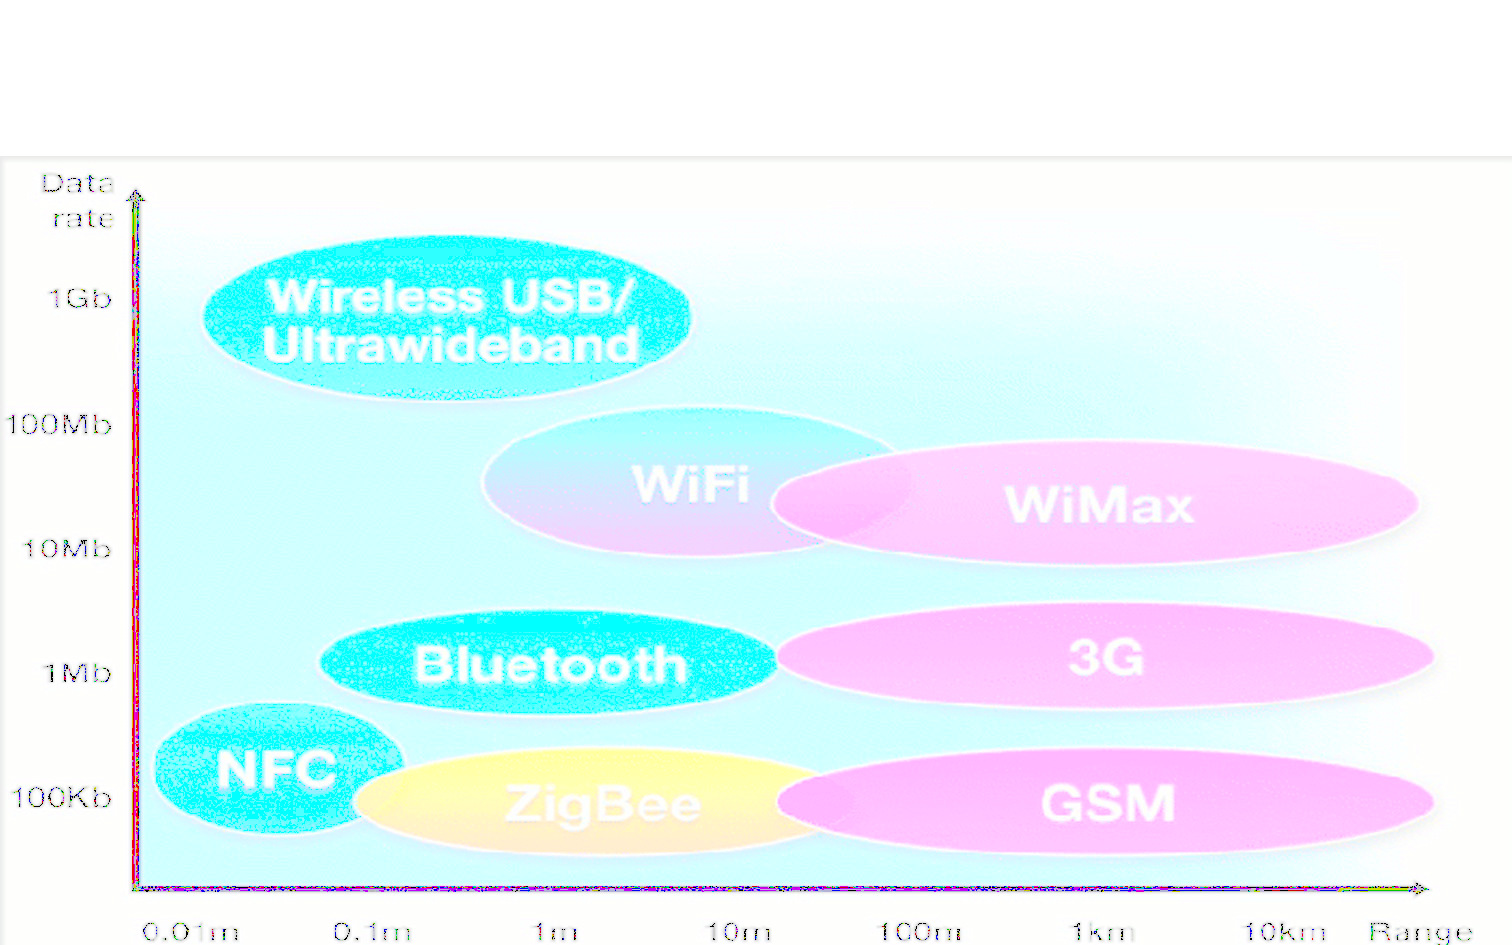
\includegraphics[width=\paperwidth,height=\paperheight,keepaspectratio]{scope_slide.jpg}}
% Start of fourth slide
\section{Objective of work} % A subsection can be created just before a set of slides with a common theme to further break down your presentation into chunks
\begin{frame} 
	\frametitle{Objective of work} 
	\begin{itemize} \color{blue} % Shows text in bullet point 
		\item \textbf{We aspired to know more about wireless communication.}	
		\item \textbf{The work shall be a systematic guide to anyone who wants to use serial communication in their projects.}
		\item \textbf{In applications like automatic car parking systems and others when used in coordination with sensors}
		\item \textbf{Different network have different standard and we can find a way to communicate between them} \color{black}
\end{itemize}

\end{frame}
}

%------------------------------------------------
\section{Scope of the work} % Sections can be created in order to organize your presentation into discrete blocks, all sections and subsections are automatically printed in the table of contents as an overview of the talk
%------------------------------------------------
% A subsection can be created just before a set of slides with a common theme to further break down your presentation into chunks
{
 \usebackgroundtemplate{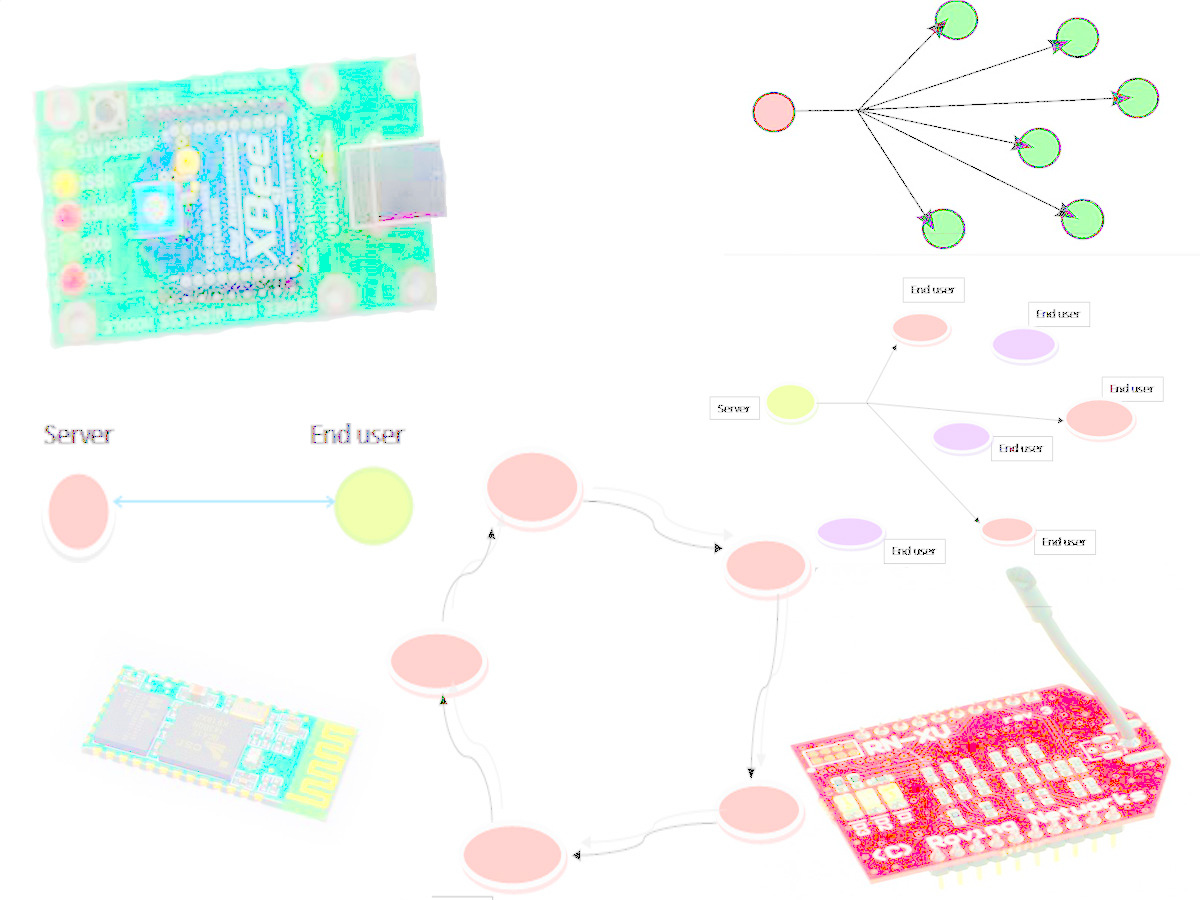
\includegraphics[height=\paperheight]{slide-1.jpg}}
% Start of Third slide
\begin{frame}
	\frametitle{Scope of work}
			\begin{itemize} 
		\item \color{red} \textbf{Zigbee}  \color{black}
		\begin{itemize}\color{blue}
			\item \textbf{communication between zigbee}
			\item \textbf{Different network configuration}
			\item \textbf{code for interfacing firebird V} \color{black}
		\end{itemize}
	\end{itemize}
 	\begin{itemize}
		\item \color{red} \textbf{Bluetooth}  \color{black}
		\begin{itemize}\color{blue}
			\item \textbf{Video tutorial for serial communication}
			\item \textbf{interfacing bluetooth in AT mode and transparent mode}\color{black}
		\end{itemize}
	\end{itemize}
	\begin{itemize}
		\item \color{red} \textbf{WiFi}  \color{black}
		\begin{itemize} \color{blue}
			\item \textbf{configuring WiFi in access point mode and interfacing mode}
			\item \textbf{Code for controlling firebird V through WiFi} \color{black}
		\end{itemize}
	\end{itemize}
\end{frame}
}
%------------------------------------------------

%------------------------------------------------
% Start of fifth slide

\section{Completion status} % A subsection can be created just before a set of slides with a common theme to further break down your presentation into chunks
\begin{frame}
\frametitle{Completion status}
\begin{columns}[c] % The "c" option specifies centered vertical alignment while the "t" option is used for top vertical alignment

\column{.45\textwidth} % Left column and width
\begin{enumerate} \color{red}
\item unicast mode \includegraphics[width=1.3cm,height=1.3cm,keepaspectratio]{unicast}
\item Broadcast 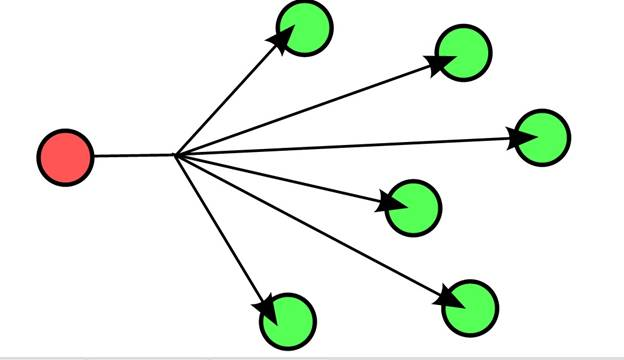
\includegraphics[width=1.3cm,height=1.3cm,keepaspectratio]{broad}
\item Serial Comm. 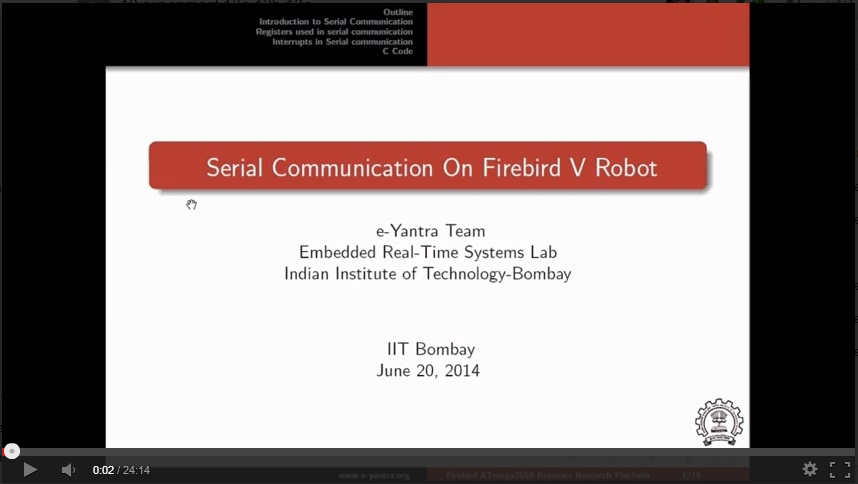
\includegraphics[width=1.3cm,height=1.3cm,keepaspectratio]{serial}
\item RFID  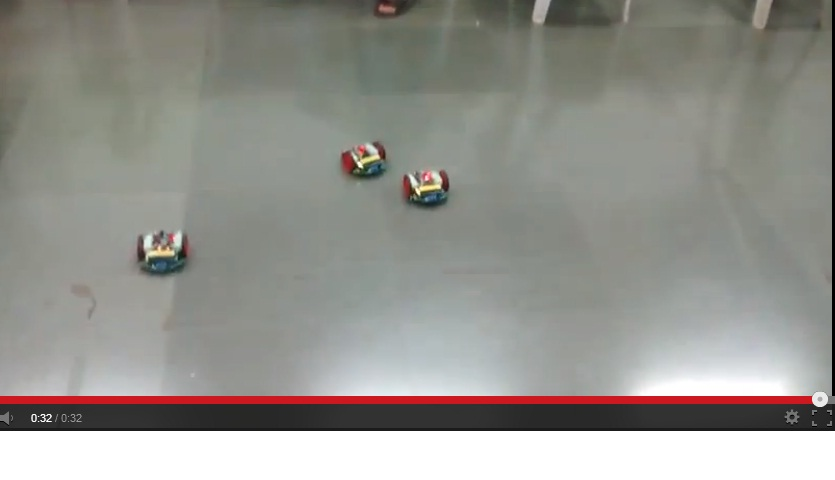
\includegraphics[width=1.3cm,height=1.3cm,keepaspectratio]{RFID}
\item Master-slave      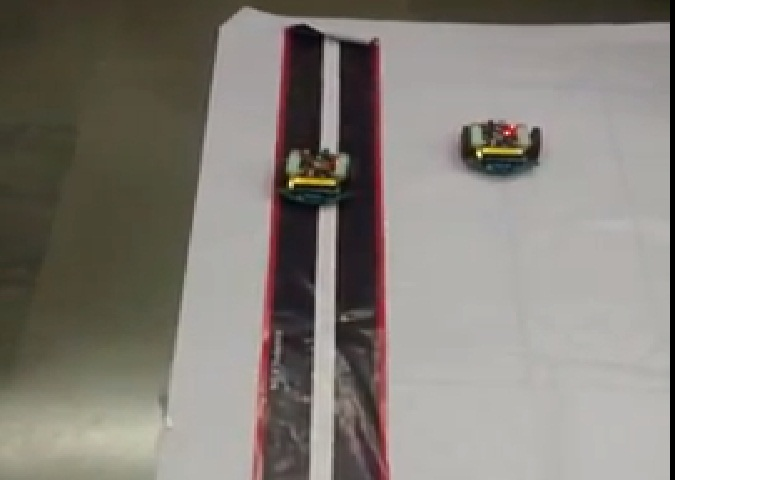
\includegraphics[width=1.3cm,height=1.3cm,keepaspectratio]{masl}
\item Zigbee book 
\includegraphics[width=1.3cm,height=1.3cm,keepaspectratio]{guide}
\item Coordination 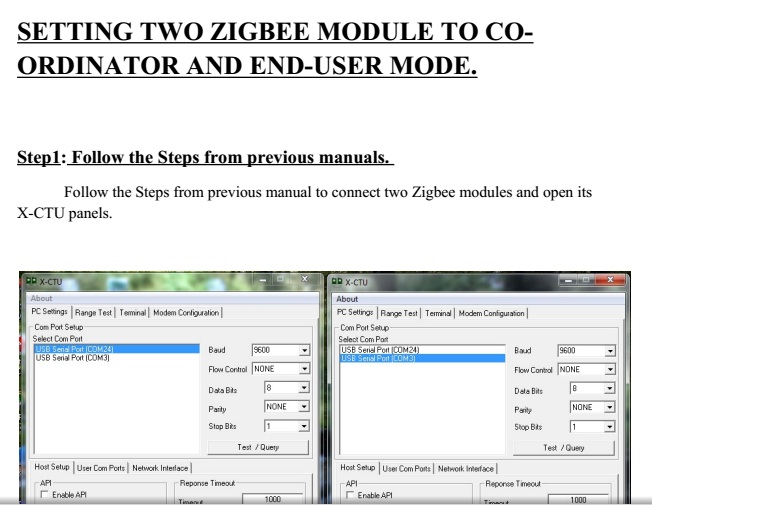
\includegraphics[width=1.3cm,height=1.3cm,keepaspectratio]{coordination} \color{black}
\end{enumerate}

\column{.5\textwidth} % Right column and width
\begin{enumerate} \color{red}
\item Dynamic Address 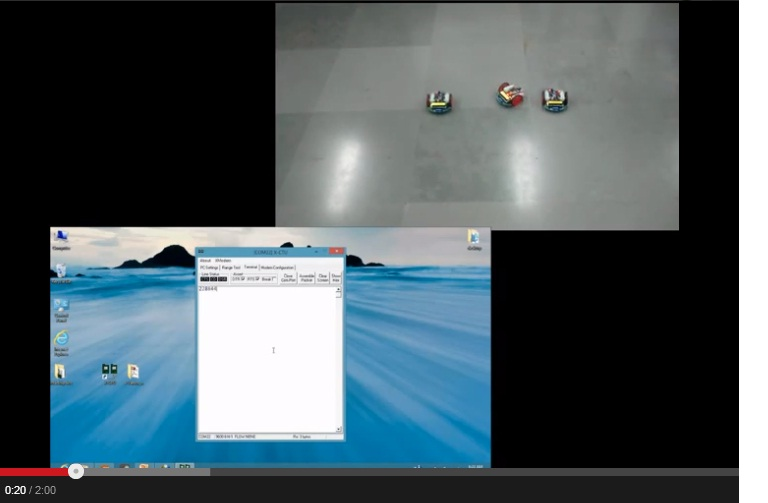
\includegraphics[width=1.3cm,height=1.3cm,keepaspectratio]{dynamic}
\item Analog-Digital data 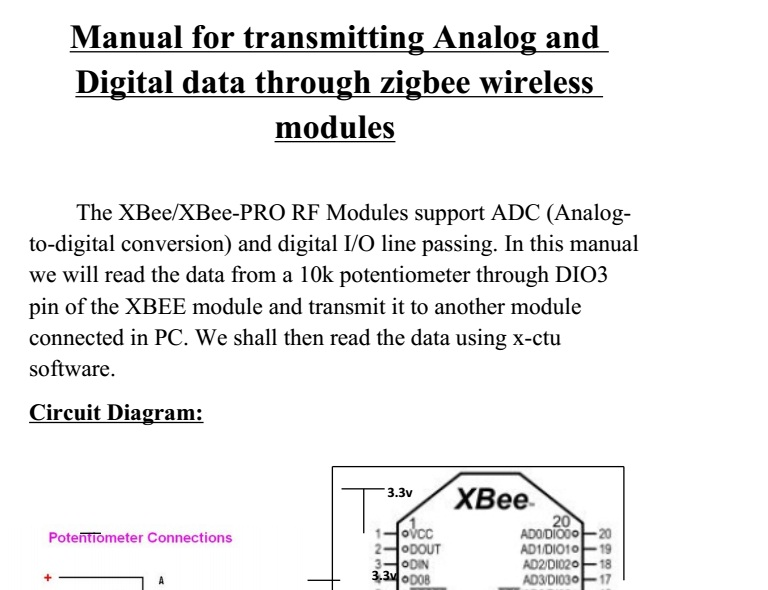
\includegraphics[width=1.3cm,height=1.3cm,keepaspectratio]{AD}
\item Ring Topology 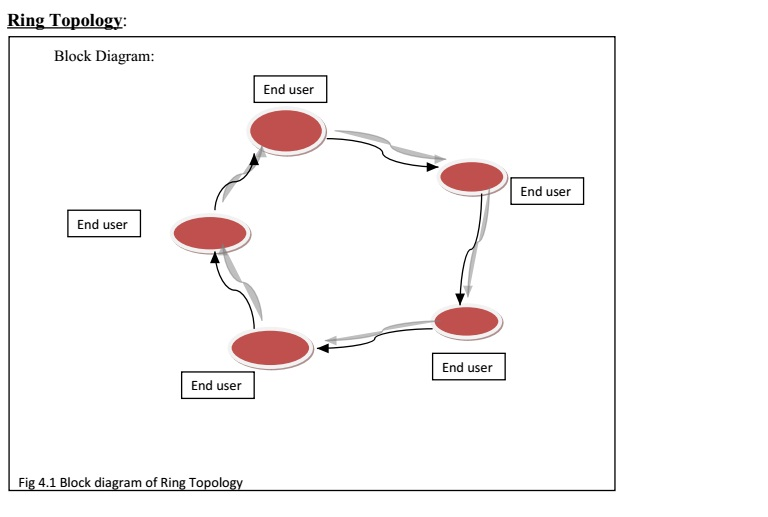
\includegraphics[width=1.3cm,height=1.3cm,keepaspectratio]{ring}
\item Bluetooth AT 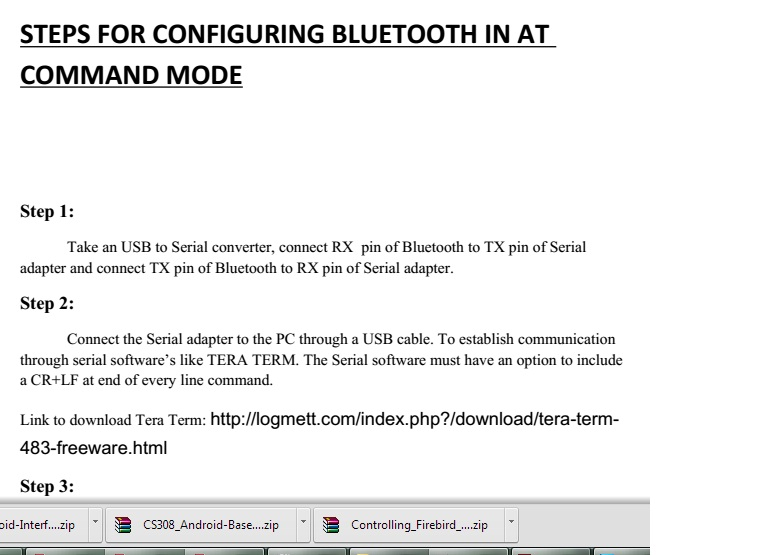
\includegraphics[width=1.3cm,height=1.3cm,keepaspectratio]{bluetooth}
\item WiFi AT AP 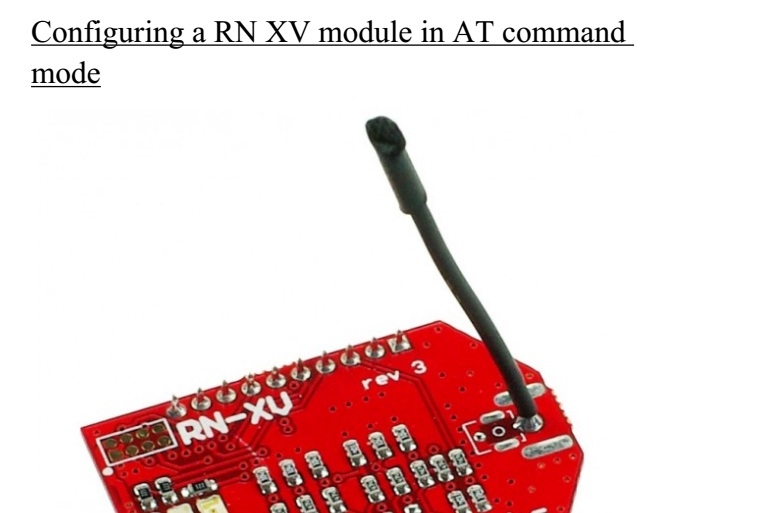
\includegraphics[width=1.3cm,height=1.3cm,keepaspectratio]{wifi}
\item WiFi FB interface 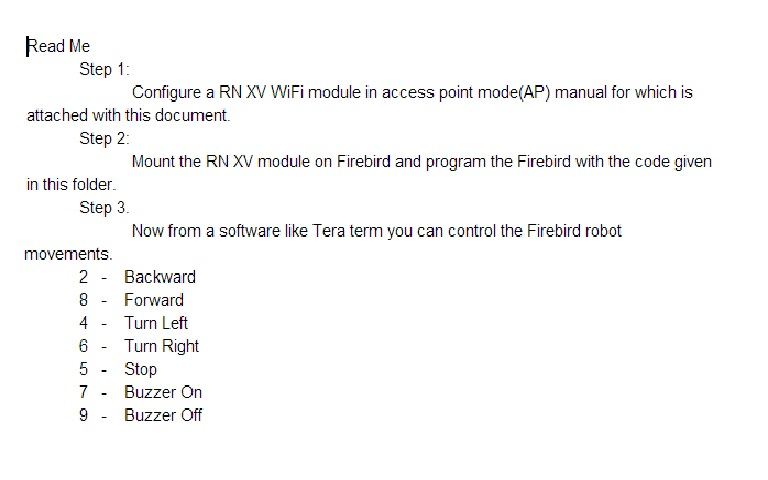
\includegraphics[width=1.3cm,height=1.3cm,keepaspectratio]{wfb} \color{black}
\end{enumerate}
\end{columns}
\end{frame}

% Start of Ninth slide

{
 \usebackgroundtemplate{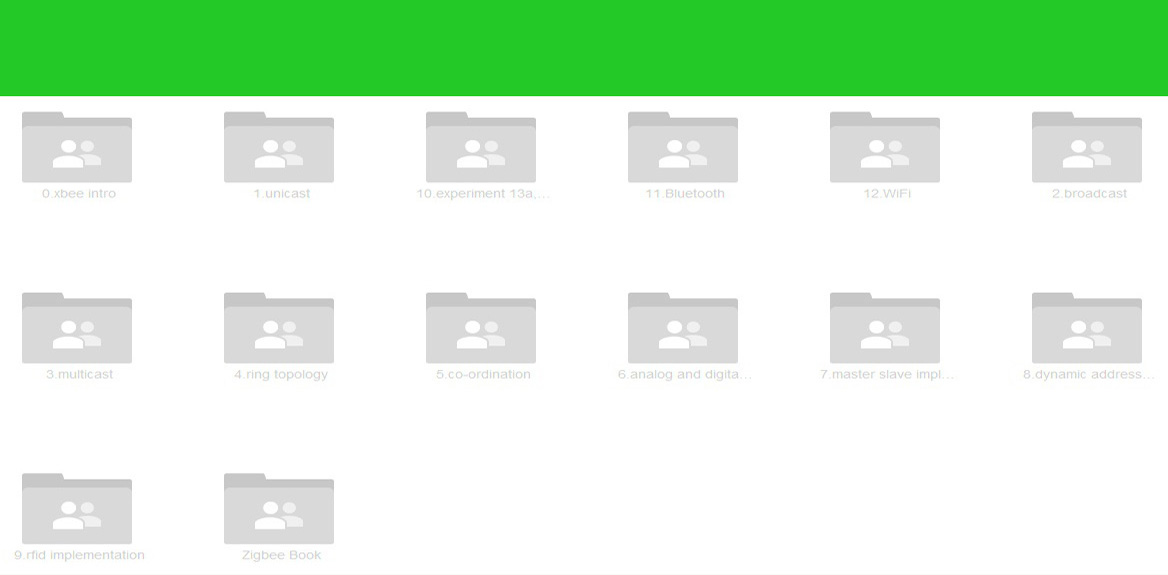
\includegraphics[height=\paperheight]{resultb}}
\section{Results and discussion} % A subsection can be created just before a set of slides with a common theme to further break down your presentation into chunks
\begin{frame}
	\frametitle{Results and discussion}
	\begin{itemize}
	\item  \color{blue} We have made a clearly understandable and step by step procedural manual and video tutorial for wireless module like Bluetooth, X-bee and Wi-Fi and serial communication.
	\item We had several application to support various configuration in x-bee but we could not implement the same for Wi-Fi and Bluetooth because we had acute shortage of time and some components failure \color{blue}
\end{itemize}	
\end{frame}
}
%------------------------------------------------
{
 \usebackgroundtemplate{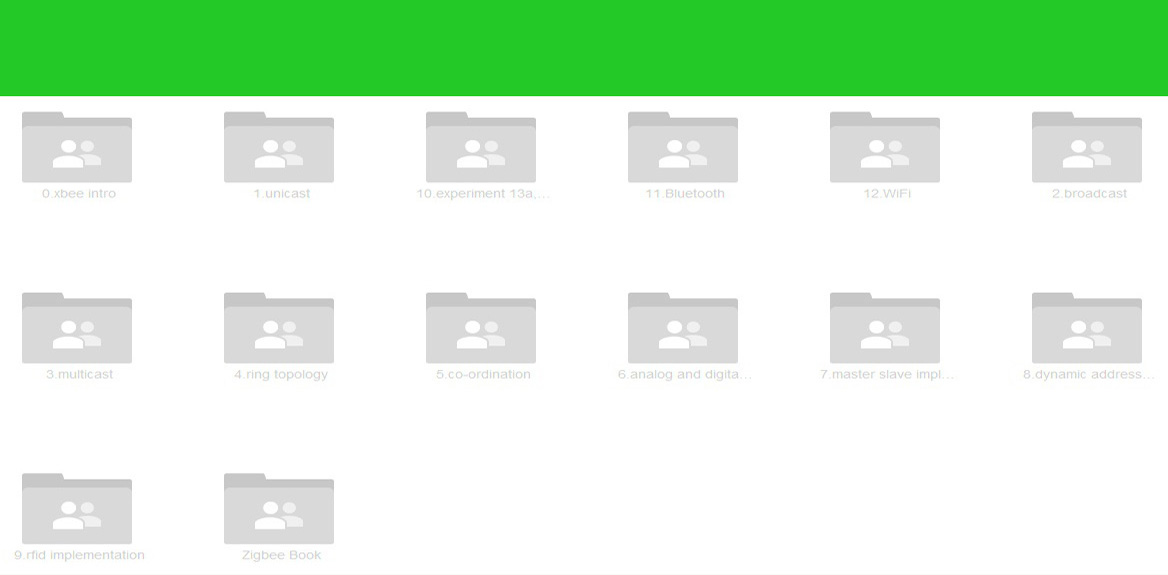
\includegraphics[height=\paperheight]{resultb}}
\section{Features and bugs} % A subsection can be created just before a set of slides with a common theme to further break down your presentation into chunks
\begin{frame}
	\frametitle{Features and bugs} \color{red}
	\textbf{Features}
	\begin{itemize} \color{blue}
		\item In case of X-bee almost all configurations are explained in detail, one need to go through this manual and video tutorial for easy understanding. This is extracted juice from various websites and manuals.
		\item In Wi-Fi and Bluetooth application are not discussed much, however various modes of configuration are explained in detail
		\item In Wi-Fi and Bluetooth application are not discussed much, however various modes of configuration are explained in detail.	
	\end{itemize}
	\textbf{Bugs}
	
\begin{itemize} \color{blue}
\item we could not extract the data sent from the Bluetooth exactly in the robot  we could receive only some Garbage value  
\end{itemize}
\color{black}
\end{frame}
}


{
 \usebackgroundtemplate{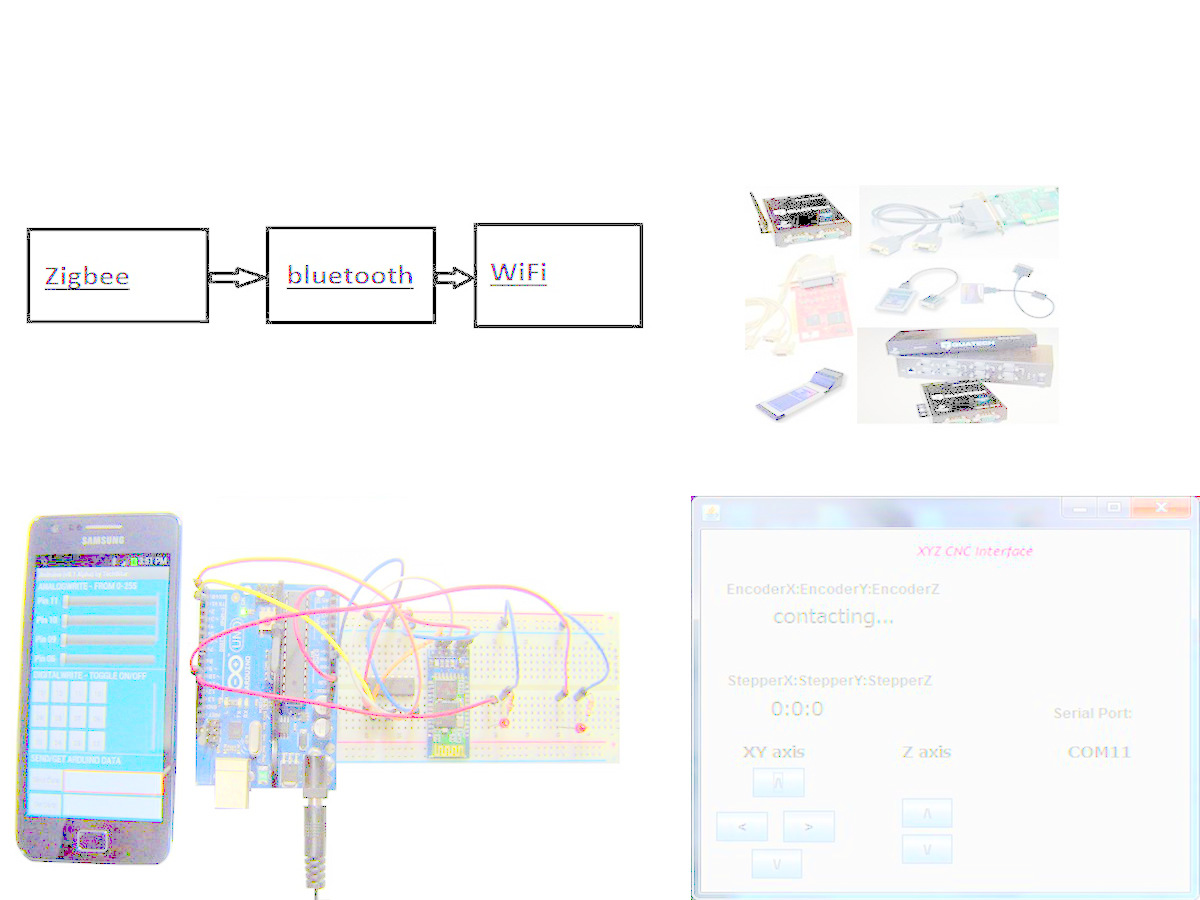
\includegraphics[height=\paperheight]{futur}}
\section{Future work} % A subsection can be created just before a set of slides with a common theme to further break down your presentation into chunks
\begin{frame}
	\frametitle{Future work} 
	\begin{itemize} \color{blue}
		\item As the configuration are explained in detail next phase would be to develop application incorporating the various configurations.
		\item We can also work on finding a coordination between various modules
		\item Study the energy consumption of these modules and using sleep, implement energy saving products for existing applications.
		\item Making a java GUI and android app on it.
	\end{itemize}
\color{black}
\end{frame}
}


\section{BE project idea}
\begin{frame}
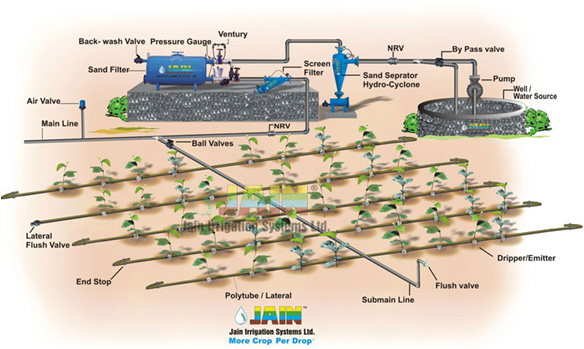
\includegraphics[width=6cm,height=6cm,keepaspectratio]{beproject}
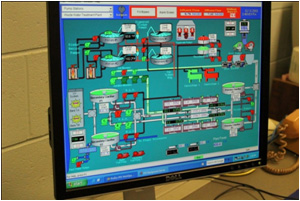
\includegraphics[width=3.5cm,height=3.5cm,keepaspectratio]{beproject2}
\end{frame}

\end{document}